\documentclass[preprint, hmargin=1in, vmargin=1in]{aastex62}
%%%%%%begin preamble
%\usepackage[hmargin=1in, vmargin=1in]{geometry} % Margins
\usepackage{hyperref}
\usepackage{url}
\usepackage{natbib}
\setlength{\bibsep}{0pt plus 0.3ex}
\usepackage{graphicx}
\usepackage{amsmath}
\usepackage{amsfonts}
\usepackage{amssymb}
%\usepackage{import}
\usepackage{wrapfig}

\usepackage{color}
\hypersetup{
  colorlinks   = true,
  %citecolor    = blue
  citecolor    = gray
  % gray is not being found!?!
  % gray is found if pdfpages is used... crap.
  %citecolor    = grey
  %citecolor    = Gray
}

%% headers
\usepackage{fancyhdr}
\pagestyle{fancy}
\fancyhf{} % sets both header and footer to nothing
\lhead{Evan Anders -- Previous \& Current Research}
\rhead{NASA Hubble Fellowship Program}
\cfoot{\footnotesize{\thepage}}
%\pagestyle{empty}
%\pagenumbering{gobble}
%\renewcommand*{\thefootnote}{\fnsymbol{footnote}}

\renewcommand{\vec}{\ensuremath{\boldsymbol}}
\newcommand{\dedalus}{\href{http://dedalus-project.org}{Dedalus}}
\newcommand{\del}{\ensuremath{\vec{\nabla}}}
\newcommand{\scrS}{\ensuremath{\mathcal{S}}}

\newcommand{\prf}{Physical Review Fluids}

\begin{document}
\begin{figure*}[t!]
	\vspace{-6pt}
	\begin{center}
    \includegraphics[width=0.9\textwidth]{./figs/snapshots_fig.pdf}
	\end{center}
	\vspace{-25pt}
    \caption{ 
	\citep[Fig.~2 of][]{anders&brown2017} Entropy perturbations in evolved convective simulations; blue is negatively buoyant while red is positively buoyant.
	(left three panels) Evolved flow structures in 2D simulations, including low Mach number (top), high Mach number (middle and bottom), and highly turbulent dynamics (bottom).
	Overall flow structures are nearly the same (large rolls) regardless of Mach number or degree of turbulence, although the high Mach number cases do exhibit shocks near the top of downflow lanes (e.g., upper left corner of middle panel).
	(right panels) Evolved flows in a 3D simulation, including a vertical cut through the domain (top) and horizontal slices near the top and (bottom left) and middle (bottom right) of the domain.
	Flows in 3D take on plume structures rather than time-stationary rolls, and the surface dynamics strikingly resemble convection at the solar surface.
	Despite very different dynamics in 2D and 3D, many properties of the overall convective flows (heat transport, turbulence) are very similar between 2D and 3D.
	\label{fig:ab17} }
	\vspace{-66pt}
\end{figure*}
\section*{\textbf{Previous Research}}
\thispagestyle{fancy}
\paragraph{Scaling Laws in Fully Compressible, Stratified Convection}
The levels of turbulence achieved by stellar convection is far beyond what can be simulated on modern computational resources \citep[see e.g.,][for a discussion]{brummell&all2002}.
This limitation means that numericists like myself aim to understand how basic measures of the flow change as the degree of turbulence is increased towards the stellar regime so that we can extrapolate out to stellar parameters.
In \citet{anders&brown2017}, I studied scaling laws in fully compressible, stratified convection.
I showed that the Mach number of convective simulations is straightforward to specify in polytropic atmospheres, and then studied how convection changes from the laminar to the turbulent regime in 2D and 3D convection.
Characteristic flow fields from these simulations are depicted in Fig.~\ref{fig:ab17}, from this paper.
We surprisingly found that stratified convection at both very low and very high Mach numbers exhibited scaling laws that were nearly identical to those seen in incompressible Boussinesq convection \citep{ahlers&all2009}.

\vspace{-4pt}
\paragraph{Fixing Rotational Constraint in Convective Simulations}
Convection in astrophysical and geophysical contexts experience Coriolis forces due to the global rotation of the star or planet on which the convection occurs.
These Coriolis forces suppress convective motions, and therefore the degree of turbulence and the degree of rotational influence in the evolved convective state is a complicated function of convective driving and global rotation.
In \citet{anders&all2019}, I extended my studies of stratified, compressible convection to include rotation.
We discovered a new parameter, the ``predictive Rossby number'' (Ro$_\text{P}$), which is informed by the convective driving and global rotation and which, when held constant, allows the degree of turbulence in convection simulations to be straightforwardly increased.
When the rotation rate or convective driving are changed on their own, the amount of rotational influence felt by the evolved convective flows either increases or decreases as turbulence is increased.
However, at a fixed value of Ro$_\text{P}$, the rotational influence felt by the evolved flows does not change with increasing turbulence.
Select figures from this work have been annotated and displayed in Fig.~\ref{fig:rossby_plot}.

\begin{figure*}[t]
	\begin{center}
    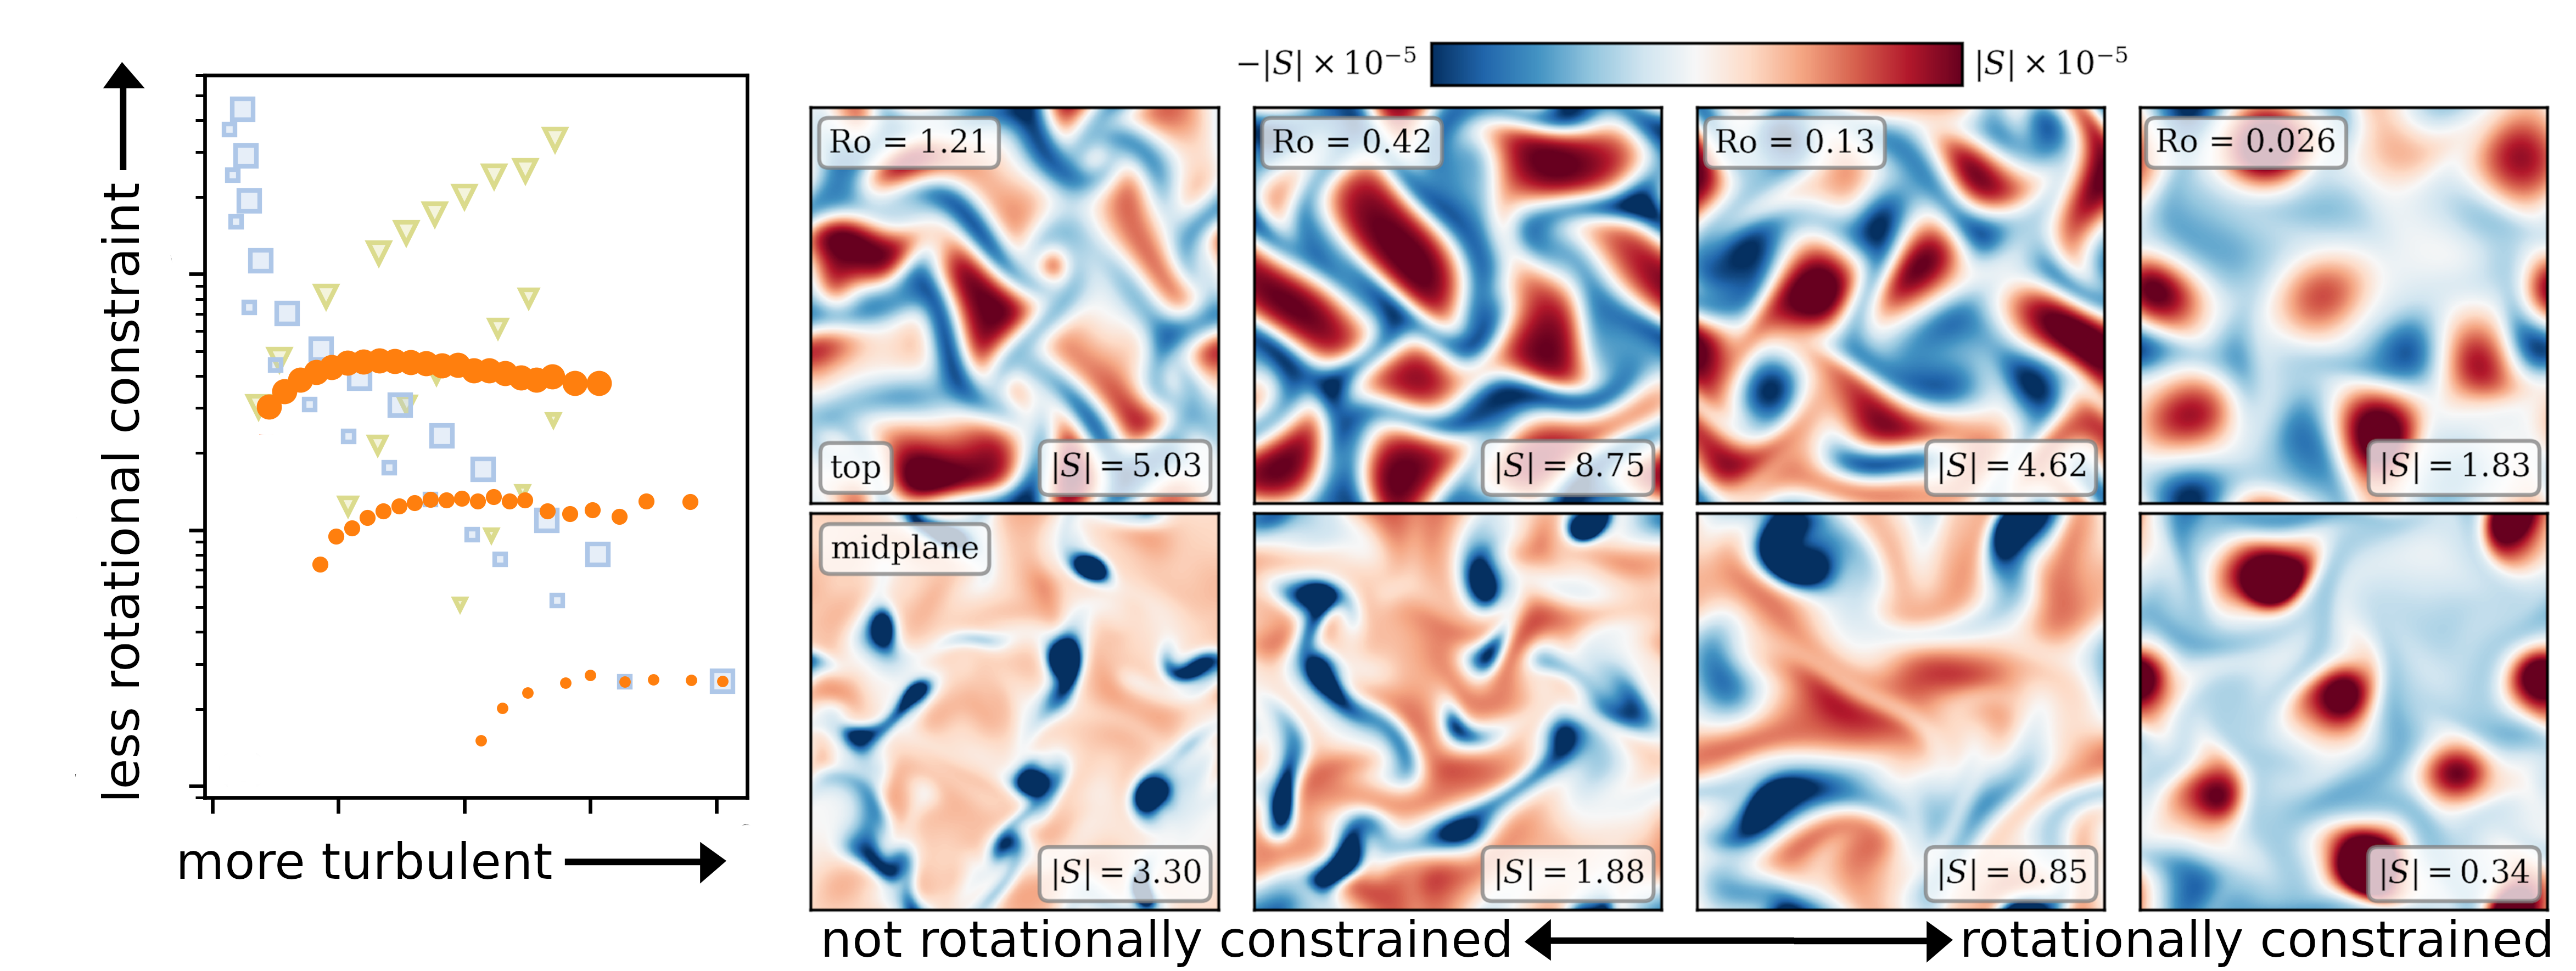
\includegraphics[width=0.9\textwidth]{./figs/rossby_plot.pdf}
	\end{center}
	\vspace{-22pt}
    \caption{ 
	\citep[From Figs.~1 \& 2 of][]{anders&brown2017} Left panel: As turbulence is increased in convective simulations, the rotational constraint felt by the flows changes along traditional paths through parameter space (green triangles and blue squares) but stays constant along our newly-found paths (orange circles).
	Right panels: As rotational constraint increases (left to right), the granular convective structures seen in e.g., Fig.~\ref{fig:ab17} give way to quasi-2D vortical columns which change very little between the top (upper row) and midplane (lower row) of the atmosphere, even in the presence of stratification.
	The very different flow structures observed when rotational constraint is important implies that it is crucial to simulate in the same regime in which an astrophysical object of interest exists.
	\label{fig:rossby_plot} }
	\vspace{-11pt}
\end{figure*}

\vspace{-11pt}
\paragraph{Accelerated Evolution of Convective Simulations}
\begin{wrapfigure}{r}{0.5\textwidth}
	\begin{center}
	\vspace{-22pt}
    \includegraphics[width=0.48\textwidth]{./figs/nu_v_time.png}
	\vspace{-16pt}
	\end{center}
    \caption{
	\citep[Fig.~2 of][]{anders&all2018} The time evolution of convective transport (black line) and thermal energy (blue line) for a simulation which uses standard timestepping (top) and one which uses our accelerated evolution method (bottom).
	Standard timestepping converges over thousands of convective timescales, but our accelerated evolution method (which occurs at the times marked by arrows) rapidly and accurately achieves the same converged state.
	\label{fig:ae_plot} }
	\vspace{-16pt}
\end{wrapfigure}
In highly turbulent simulations of astrophysical convection, the timescale over which the atmospheric stratification evolves (e.g, the Kelvin-Helmholtz [KH] timescale) is much larger than the timescale on which convective motions overturn.
However, in order to have faith in the results of convective simulations, it is crucial to timestep through at least one KH timescale to ensure that simulation results are in a statistical equilibrium.
This means that a vast amount of computational resources are often ``wasted'' equilibrating simulations before meaningful measurements can be made.
In \citet{anders&all2018}, I studied and verified a tool for accelerating through the long thermal relaxation of convective atmospheres.
In a simplified convective system, this tool equilibrated a solution to within 1\% accuracy of traditional timestepping techniques while using an order of magnitude fewer resources.
Time traces comparing properties of a traditional simulation to one of these accelerated simulations are shown in Fig.~\ref{fig:ae_plot}.


\vspace{-4pt}
\paragraph{Entropy Rain: Thermals as Downflows in Stellar Convection}
\begin{wrapfigure}{l}{0.5\textwidth}
	\begin{center}
	\vspace{-33pt}
    \includegraphics[width=0.48\textwidth]{./figs/evolution_colormeshes.pdf}
	\vspace{-16pt}
	\end{center}
    \caption{
	\citep[Fig.~2 of][]{andersLB2019} Shown is the evolution of the entropy signature in a vertical slice through thermals in weakly stratified (left) and highly stratified (right) atmospheres.
	In the presence of weak stratification, these downflows grow with depth; in the presence of strong stratification, they are compressed and they accelerate as they propagate downwards.
	\label{fig:thermals} }
	\vspace{-22pt}
\end{wrapfigure}
Most recently, I have studied the effects of atmospheric stratification on individual convective downflows.
I model downflows as ``thermals,'' or cold regions of fluid which naturally evolve due to buoyancy forces, which are studied extensively in the Earth's atmosphere \citep{lecoanet&jeevanjee2019}.
The evolution of thermals in minimally stratified and appreciably stratified domains is depicted in Fig.~\ref{fig:thermals}.
In \citet{andersLB2019}, I developed an analytical theory for the size of these downflows as a function of atmospheric depth, and I verified that theory with simulations. 
Stratification compresses these downflows as the density increases, but not as much as a simple estimate based on the density profile would suggest \citep[as in][]{brandenburg2016}.
We find that downflows in the Sun remain large enough to shield their entropy signature from dissapative effects and transport enough energy to carry the solar luminosity alone.


\section*{\textbf{Current Research}}
As I finish my PhD, I am extending my research to three small collaborative projects which build upon these results.

\vspace{-4pt}
\paragraph{Individual downflows impinging on stable layers}
Alongside Prof.~Daniel Lecoanet (Northwestern / Princeton) and Dr.~Lydia Korre (Univ.~Colorado), I am extending my Entropy Rain study to include interactions with the stable layer that lies beneath a solar-like convection zone.
While there have been many simple studies of the interactions of thermals with stable regions of fluid in the laboratory over the past few decades, few studies have focused on where the buoyant energy signature of the flow is deposited.
In the Sun, the location of this energy deposition could have huge implications on observed convective dynamics.
For example, cold downflow material deposited at the base of the convection zone could strongly stabilize that region and suppress flows from being driven there \citep{cossette&rast2017}.

\vspace{-4pt}
\paragraph{Thermal Relaxation and Dynamical Regime changes}
During my PhD, I learned how to set the degree of rotational constraint in a rotating convection simulation and I learned how to fast-forward through thermal relaxation.
I am collaborating with Prof.~Geoff Vasil (Univ.~Sydney) to study the effects of thermal relaxation on convective simulations where complicating effects like rotation are included in order to demonstrate the importance of achieving a relaxed state.
We have found that at highly turbulent, astrophysically-interesting parameters, the degree of rotational constraint felt by convective flows can change by an order of magnitude between a transient and fully relaxed solution.
These results suggest that simulations in certain regimes which do not carefully achieve thermal equilibration may sample completely nonsensical convective dynamics.

\vspace{-4pt}
\paragraph{Predicting the Rossby number in global simulations}
The final project I am collaborating on as I finish up my PhD is one with Dr.~Nick Featherstone (Univ.~Colorado).
The simulations I conducted in \citet{anders&brown2019} showed that the degree of rotational constraint could be set \emph{a priori} in \emph{Cartesian} simulations of rotating convection.
Dr.~Featherstone and I are currently investigating whether or not this can be achieved in convective simulations in spherical geometries.
Past work by \citet{featherstone&hindman2016} shows that the degree of rotational constraint felt by convective flows in a global simulation can vastly change the evolved flow structures, and so verifying our mechanism in global simulations is crucial.


\bibliographystyle{../yahapj}
\bibliography{../biblio}
\end{document}
